\documentclass[a4paper,11pt]{book}
\renewcommand{\familydefault}{\sfdefault}

\usepackage{standalone}
\usepackage[english]{babel}
\usepackage[top=3cm]{geometry}
\usepackage{float}
\usepackage{tabularx}
\usepackage{multirow}
\usepackage{booktabs}
\usepackage{pgfplots}
\usepackage{amsmath}
\usepackage{amssymb}
\usepackage{amsfonts}
\usepackage{siunitx}
\usepackage{tikz}
\usepackage{graphics} % for pdf, bitmapped graphics files
\usepackage{graphicx}
\usepackage{exsheets}
\usepackage{algorithm}
\usepackage{algorithmicx}
\usepackage[noend]{algpseudocode}
\usepackage{hyperref}
\usepackage{enumitem}
\usepackage{filecontents}
\usepackage{multirow}
%\usepackage{showframe}% to show frames
%\ifCLASSOPTIONcompsoc
\usepackage[caption=false, font=normalsize, labelfont=sf, textfont=sf]{subfig}
%\else
%\usepackage[caption=false, font=footnotesize]{subfig}
%\fi    

\usetikzlibrary{patterns,arrows,arrows.meta,calc,intersections,shapes,positioning,decorations.pathreplacing,decorations.markings,decorations.pathmorphing}
\usepackage{multicol}

\sisetup{output-decimal-marker={,},exponent-product=\cdot}

\DeclareSIUnit\atm{atm}
\DeclareSIUnit\dioptre{D}



\def\BState{\State\hskip-\ALG@thistlm}


\definecolor{TitleColor}{rgb}{0.65,0.04,0.07}
\definecolor{NumberColor}{rgb}{0.02,0.04,0.48}

\DeclareInstance{exsheets-heading}{fancy}{default}{
toc-reversed = true ,
indent-first = true ,
vscale = 2 ,
pre-code = \IfInsideQuestionT{\rule{\linewidth}{1pt}} ,
post-code =\IfInsideQuestionT{\rule{\linewidth}{1pt}} ,
subtitle-format = \large\scshape\color{rgb:red,0.65;green,0.04;blue,0.07} ,
number-format = \large\bfseries\color{rgb:red,0.02;green,0.04;blue,0.48} ,
points-format = \itshape ,
join = { number[r,B]title[l,B](.333em,0pt);
title[r,B]subtitle[l,B](1em,0pt)
} ,
attach =
{
main[hc,vc]number[hc,vc](0pt,0pt) ;
main[l,vc]subtitle[hc,vc](\marginparsep,0pt)
}
}



\DeclareInstance{exsheets-heading}{block-subtitle}{default}{
vscale = 2 ,
pre-code = \rule{\linewidth}{1pt} ,
post-code = \rule{\linewidth}{1pt} ,%title-format = \large\scshape\color{TitleColor} ,
number-format = \large\bfseries\color{rgb:red,0.02;green,0.04;blue,0.48} ,
subtitle-format = \large\scshape\color{black} ,
join = {
title[r,B]number[l,B](.333em,0pt) ;
title[r,B]subtitle[l,B](1em,0pt)
} ,
attach = {
main[l,vc]title[l,vc](0pt,0pt) ;
main[r,vc]points[l,vc](\marginparsep,0pt)
},
}

\DeclareQuestionClass{textbook}{textbooks}

\SetupExSheets{
  headings = fancy,
  question/print = true ,
  solution/print = false }
 % counter-format = se.qu ,
%  counter-within = section ,
  %question/pre-hook = \rule{\textwidth}{1pt},


\hypersetup{
	colorlinks = true, 
	breaklinks = true, 
	bookmarks = true,
	bookmarksnumbered = true,
	urlcolor = blue, 
	linkcolor = blue, 
	citecolor=blue,
	linktoc=page, 
	pdftitle={}, 
	pdfauthor={\textcopyright Author}, 
	pdfsubject={}, 
	pdfkeywords={}, 
	pdfcreator={pdfLaTeX}, % PDF Creator
	pdfproducer={IEEE} }





\tikzset{point/.style={circle,fill,black!80,inner sep=0pt,minimum size=#1,opacity=0.9}}
\tikzset{point/.default=3pt}\tikzset{vector/.style={line width=1pt,postaction={decorate,decoration={markings,mark=at position 1 with {\arrow{latex}}}}}}
\tikzset{block/.style={rectangle,fill=black!30,draw,minimum size=#1,opacity=0.9,align=center}}
\tikzset{block/.default=15pt}\tikzset{ball/.style={circle,fill=black!30,draw,minimum size=#1,opacity=0.9}}
\tikzset{ball/.default=5pt}\tikzset{pulley/.style={draw=black,line width=0.2pt,circle,minimum size=#1,inner sep=0pt,fill=black!10}}
\tikzset{pulley/.default=20pt}\tikzset{rod/.style={line width=2pt}}
\tikzset{rope/.style={line width=1pt}}
\tikzset{spring/.style={decorate,decoration={coil,amplitude=5pt,segment length=#1,aspect=0.3}}}
\tikzset{spring/.default=5pt}\tikzset{wall/.style={black!10,pattern=north east lines,opacity=0.3}}
\tikzset{ray/.style={line width=0.8pt,postaction={decorate,decoration={markings,mark=at position 0.5 with {\arrow{>}}}}}}
\tikzset{arrow/.style={-latex}}
\tikzset{object/.style={line width=1pt,orange,-latex}}
\tikzset{image/.style={line width=1pt,blue,-latex}}
\tikzset{doublearrow/.style={<->,>=latex,thick}}
\tikzset{brace/.style={decorate,decoration={brace,amplitude=#1}}}
\tikzset{brace/.default=5pt}




\graphicspath{{images/}} 




\makeatletter
\@addtoreset{question}{section}
\makeatother


\begin{document}
\author{Dr. Muhammed Rushdi \and Asem Alaa}

\title{Measurements and Instrumentation [SBE206A] (Fall 2018)\\ Tutorial 1}

\maketitle

\chapter*{Cheat Sheet}
\tikzstyle{mybox} = [draw=black, fill=white, very thick,
    rectangle, rounded corners, inner sep=10pt, inner ysep=10pt]
\tikzstyle{fancytitle} =[fill=black, text=white, font=\bfseries]
%\newcommand*\bigcdot{\mathpalette\bigcdot@{.5}}
%\newcommand*\bigcdot@[2]{\mathbin{\vcenter{\hbox{\scalebox{#2}{$\m@th#1\bullet$}}}}}

\begin{multicols*}{2}


%------------ Length ---------------
\begin{tikzpicture}
\node [mybox] (box){%
    \begin{minipage}{0.3\textwidth}
    ${\rm 1 m = 3.2808 ft }$ \\
    ${\rm 1 km = 0.621 mi }$ 
    \end{minipage}
};
\node[fancytitle, right=10pt] at (box.north west) {Length};
\end{tikzpicture}

%------------ Volume ---------------
\begin{tikzpicture}
\node [mybox] (box){%
    \begin{minipage}{0.3\textwidth}
    ${\rm 1 L = 0.001 m^3 }$\\
    ${\rm 1 L = 61.02 in.^3}$
    \end{minipage}
};
\node[fancytitle, right=10pt] at (box.north west) {Volume};
\end{tikzpicture}

%------------ MASS ---------------
\begin{tikzpicture}
\node [mybox] (box){%
    \begin{minipage}{0.3\textwidth}
    ${\rm 1 kg = 2.2046 lbm }$\\
    ${\rm 1 kg  = 0.068 522 slug }$
    \end{minipage}
};
\node[fancytitle, right=10pt] at (box.north west) {Mass};
\end{tikzpicture}


%------------ Force ---------------
\begin{tikzpicture}
\node [mybox] (box){%
    \begin{minipage}{0.3\textwidth}
    ${\rm 1 N = 0.2248 lbf }$
    \end{minipage}
};
\node[fancytitle, right=10pt] at (box.north west) {Force};
\end{tikzpicture}


%------------ Work/Energy ---------------
\begin{tikzpicture}
\node [mybox] (box){%
    \begin{minipage}{0.3\textwidth}
    ${\rm 1 kJ = 737.562 ft \cdot lbf  }$ \\
    ${\rm 1 kJ = 0.947 817 Btu }$
    \end{minipage}
};
\node[fancytitle, right=10pt] at (box.north west) {Work/Energy};
\end{tikzpicture}


%------------ Pressure/Stress ---------------
\begin{tikzpicture}
\node [mybox] (box){%
    \begin{minipage}{0.3\textwidth}
    ${\rm 1 atm = 14.696 psi }$ \\
    ${\rm 1 atm = 101 325 Pa }$ \\
    ${\rm 1 atm = 407.189 in. H_2O }$ \\ 
    ${\rm 1 atm = 760.00 mm Hg }$ \\ 
    ${\rm 1 atm = 1 bar }$
    \end{minipage}
};
\node[fancytitle, right=10pt] at (box.north west) {Pressure/Stress};
\end{tikzpicture}


%------------ Density ---------------
\begin{tikzpicture}
\node [mybox] (box){%
    \begin{minipage}{0.3\textwidth}
    ${\rm 1 slug/ft^3 = 512.38 kg/m^3  }$ 
    \end{minipage}
};
\node[fancytitle, right=10pt] at (box.north west) {Density};
\end{tikzpicture}

%------------ Temperature ---------------
\begin{tikzpicture}
\node [mybox] (box){%
    \begin{minipage}{0.3\textwidth}
    ${\rm K = ° C +273.15  }$ \\
    ${\rm K = (5/9) × ° F + 255.38  }$ \\
    ${\rm K = (5/9) × ° R  }$ \\
    ${\rm ° F = (9/5) × ° C + 32.0  }$ \\
	${\rm ° F = ° R - 459.69 }$
    \end{minipage}
};
\node[fancytitle, right=10pt] at (box.north west) {Temperature};
\end{tikzpicture}

%------------ Scales ---------------
\begin{tikzpicture}
\node [mybox] (box){%
    \begin{minipage}{0.3\textwidth}
    ${\rm yotta (Y) = 10^{24}  }$ \\
    ${\rm zeta (Z) = 10^{21}  }$ \\
    ${\rm exa (E) = 10^{18}  }$ \\
    ${\rm peta (P) = 10^{15}  }$ \\
    ${\rm tera (T) = 10^{12}  }$ \\
    ${\rm giga (G) = 10^{9}  }$ \\
    ${\rm mega (M) = 10^{6}  }$ \\
    ${\rm kilo (k) = 10^{3}  }$ \\
    ${\rm hecto (h) = 10^{2}  }$ \\
    ${\rm deka (da) = 10^{1}  }$ \\
    ${\rm deci (d) = 10^{-1}  }$ \\
    ${\rm centi (c) = 10^{-2}  }$ \\
    ${\rm milli (m) = 10^{-3}  }$ \\
    ${\rm micro (\mu) = 10^{-6}  }$ \\
    ${\rm nano (n) = 10^{-9}  }$ \\
    ${\rm pico (p) = 10^{-12}  }$ \\
    ${\rm femto (f) = 10^{-15}  }$ \\
    ${\rm atto (a) = 10^{-18}  }$ \\
    ${\rm zepto (z) = 10^{-21}  }$ \\
    ${\rm yocto (y) = 10^{-24}  }$ \\
    \end{minipage}
};
\node[fancytitle, right=10pt] at (box.north west) {Temperature};
\end{tikzpicture}

\end{multicols*}


\chapter*{Physical Units}

\begin{question}[subtitle=Patrick F. Dunn Sol. 2.4]
Which of the following is not equivalent to the SI unit of energy?

\begin{enumerate}
\item ${\rm kg \cdot m^2 /s^2}$
\item ${\rm Pa \cdot m^2}$
\item ${\rm N \cdot m}$
\item ${\rm W \cdot s } $
\end{enumerate}
\examspace*{5em}

\end{question}
\begin{solution}
${\rm Pa \cdot m^2}$ \\
${\rm Pa = N/m^2}$, which implies that ${\rm Pa \cdot m^2 = N}$. A newton is a unit of force, not of energy.

\end{solution}


\begin{question}[subtitle=Patrick F. Dunn Sol. 2.7]
An astronaut weighs 164 pounds on Earth (assume that Technical English is spoken). What is the astronaut’s weight (in the appropriate SI unit and
with the correct number of significant figures) on the surface of Mars where the gravitational acceleration is 12.2 feet per second squared?
\examspace*{5em}

\end{question}
\begin{solution}
276 N \\
If weight is known in one gravitational field, then the weight of the same
mass in another gravitational field can be determined simply by multiplying by the ratio of gravitational accelerations. So, multiply the weight by 12.2/32.174 to the weight on Mars. Then multiply by 4.448 N/lbf.

\end{solution}

\begin{question}[subtitle=Patrick F. Dunn Sol. 2.8]
An astronaut weighs 162 pounds on Earth (assume that Technical En-
glish is spoken). What is the astronaut’s mass (expressed in the appropriate SI unit and with the correct number of significant figures) on the surface of Mars, where the gravitational acceleration is 12.2 feet per second squared?
\examspace*{5em}

\end{question}
\begin{solution}
73.5 kg \\
There are three significant figures. To determine the mass, first convert
the weight to mass by dividing by 32.174 to get slugs. Then use the conversion 14.594 kg = 1 slug.

\end{solution}

\begin{question}[subtitle=Patrick F. Dunn Sol. 2.10]
A robotic manipulator weighs 393 lbf (Technical English) on Earth.
What is the weight of the probe on the moon’s surface in newtons (to the nearest tenth of a newton) if the lunar gravitational acceleration is 1/6 of that on Earth?
\examspace*{5em}

\end{question}
\begin{solution}
291 N \\ 
To arrive at the probe weight on the moon, multiply the weight on earth
by 1/6. Convert to newtons by multiplying by 4.448 N/lbf.


\end{solution}



\begin{question}[subtitle=Patrick F. Dunn Sol. 2.11]
How much work is required to raise a 50 g ball 23 in. vertically upward?
Express your answer in units of ft-lbf to the nearest one-thousandth of a ft-lbf.
\examspace*{5em}

\end{question}
\begin{solution}
0.211 ft-lbf \\ 
Work is force times distance. Mass and distance are given. Force is mass
times acceleration. So, the answer is \\
${\rm mass(g) \times \frac{1 kg}{1000 g} \times 9.806650 m / s^2 \times distance(in.) \times \frac{1 ft}{12 in.} \times \frac{1 m }{3.2808 ft} \times \frac{0.737562 ft-lbf}{ N \cdot m}}$


\end{solution}




\chapter*{Significant Figures}
\section*{Rationale}

\begin{itemize}

\item The number of significant figures \textit{is the number of digits between and including the least
and \emph{the most significant digits}}. 
\item The leftmost nonzero digit is called \emph{the most significant digit}; the rightmost nonzero digit, \emph{the least significant digit}.
\item If there is a decimal point in the number, then the rightmost digit is \emph{the least significant digit} even if it is a zero. 
\item These rules imply that the following
numbers have five significant figures:
\begin{itemize}
\item 1.0000
\item 2734.2
\item 53 267.
\item 428 970
\item 10 101
\item 0.008 976 0
\end{itemize} 

\end{itemize}

\subsection*{Round-off}

\begin{enumerate}
\item To round off a number, the number first is truncated to its desired length. Then the excess digits are expressed as a decimal fraction.
\item If it is greater than 1/2, we round up the least significant digit by one; if it is
less than 1/2, it is left alone. If the fraction equals 1/2, the least significant
digit is rounded up by one only if that digit is odd (Patrick F. Dunn).
\item Do not round-off intermediate results. Only the final results to be rounded-off.
\item The number of significant figures in a computed result equals the minimum number of significant figures in any number used in the computation.
\end{enumerate}


\subsection*{Scientific Notation}

\begin{itemize}
\item What happens when no decimal point is present, a zero is the rightmost digit and it is significant? This situation is ambiguous and can be avoided by expressing the number in scientific notation, where $428 970$ becomes $4.289 70 \times 10^5$ .
\item All of the digits present in scientific notation are significant. 
\end{itemize}

\begin{question}
Round off the following numbers to three significant figures: $23 421$,
$16.024$, $273.61$, $5.6850 \times 10^3$ , and $5.6750 \times 10^3$ .
\examspace{5em}

\end{question}
\begin{solution}
The answers are $23 400$, $16.0$, $274$, $5.68 \times 10^3$ , and $5.68 \times 10^3$ . Note that
$16.024$ when rounded off to three significant figures is $16.0$, where the 0 is significant
because it is to the right of the decimal point. Also note that the last two numbers
when rounded off to three significant figures become the same. This is because of our
rule for round-off when the truncated fraction equals 1/2.

\end{solution}


\begin{question}
How many significant figures does the number 001 001.0110 have?
\examspace{5em}

\end{question}
\begin{solution}
8. The left-most 2 zeros are not significant. However, the right-most zero is
significant because of the presence of a decimal point.

\end{solution}


\begin{question}
Determine in the appropriate SI units the value with the correct number
of significant figures of the work done by a $1.460 \times 10^6$ lbf force over a $2.3476$ m
\examspace{5em}

\end{question}
\begin{solution}
There are four significant figures for the force and five for the distance.
Because work is the product of force and distance (assuming that the force is applied
along the direction of motion), work will have four significant figures. The SI unit of
work is the joule, where $J = N \cdot m$. Now $1.460 \times 10^6$ lbf equals $6.495 \times 10^6 N$. So, the
work is $1.525 \times 10^6 J$ or $1.525 MJ$.

\end{solution}

\chapter*{Warming-up Circuits}

\begin{question}

Referring to Figure \ref{fig:wheatstone}, prove the following equation

\begin{equation} \label{eq:1}
 {\rm E_0 = E_i \left[ \frac{R_1}{R_1+R_2} - \frac{R_3}{R_3+R_4} \right]}
\end{equation}

Also, derive the balanced equation 
\begin{equation} \label{eq:2}
 {\rm \frac{R_1}{R_2} = \frac{R_3}{R_4} }
\end{equation}

\begin{figure}[t!]
\centering
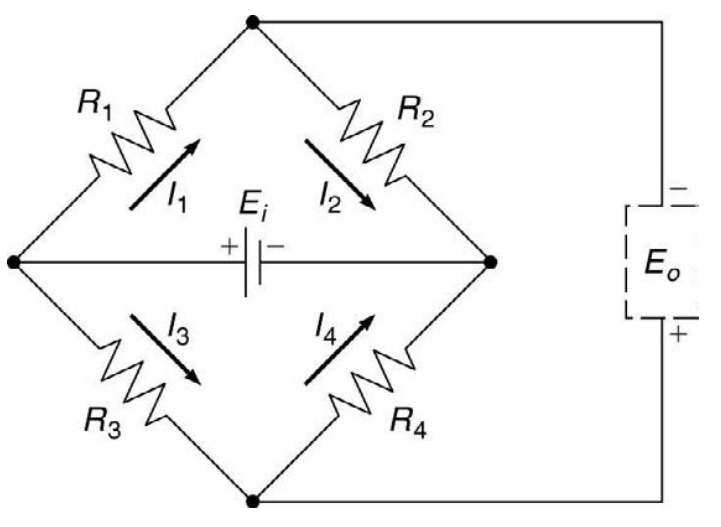
\includegraphics[scale=0.6]{wheatstone}
\caption{A wheatstone bridge.}\label{fig:wheatstone}
\end{figure}
\examspace{8em}

\end{question}
\begin{solution}

\end{solution}


\begin{question}

Referring to Figure \ref{fig:wheatstone}, if ${\rm R_1 = 1 \Omega}$, ${\rm R_2 = 3 \Omega}$, and ${\rm R_3 = 2 \Omega}$,
determine (a) the value of ${\rm R_4}$ such that the Wheatstone bridge is balanced, and (b) the bridge’s output voltage under this condition.

\end{question}
\begin{solution}

Equation \ref{eq:2} specifies the relationship between resistances when the bridge is balanced. Thus, $R_4 = \frac{R_2 R_3}{R_1} = 3 \times 2 / 1 = 6 \Omega$. Because the bridge is balanced, its output voltage is zero. This can be verified by substituting the four resistance values into Equation \ref{eq:1}.

\end{solution}

\end{document}

